%-------------------------
% Resume in Latex
% Author : Jonathan Oktaviano Frizzy
% License : MIT
%------------------------

\documentclass[letterpaper,11pt]{article}

\usepackage{latexsym}
\usepackage[empty]{fullpage}
\usepackage{titlesec}
\usepackage{marvosym}
\usepackage[usenames,dvipsnames]{color}
\usepackage{verbatim}
\usepackage{enumitem}
\usepackage[hidelinks]{hyperref}
\usepackage{fancyhdr}
\usepackage[english]{babel}
\usepackage{tabularx}
\usepackage{hyphenat}
\usepackage{fontawesome}
\usepackage{graphicx}
\input{glyphtounicode}


%---------- FONT OPTIONS ----------
% sans-serif
% \usepackage[sfdefault]{FiraSans}
% \usepackage[sfdefault]{roboto}
% \usepackage[sfdefault]{noto-sans}
% \usepackage[default]{sourcesanspro}

% serif
% \usepackage{CormorantGaramond}
% \usepackage{charter}


\pagestyle{fancy}
\fancyhf{} % clear all header and footer fields
\fancyfoot{}
\renewcommand{\headrulewidth}{0pt}
\renewcommand{\footrulewidth}{0pt}

% Adjust margins
\addtolength{\oddsidemargin}{-0.5in}
\addtolength{\evensidemargin}{-0.5in}
\addtolength{\textwidth}{1in}
\addtolength{\topmargin}{-.5in}
\addtolength{\textheight}{1.0in}

\urlstyle{same}

\raggedbottom
\raggedright
\setlength{\tabcolsep}{0in}

% Sections formatting
\titleformat{\section}{
  \vspace{-4pt}\scshape\raggedright\large
}{}{0em}{}[\color{black}\titlerule \vspace{-5pt}]

% Ensure that generate pdf is machine readable/ATS parsable
\pdfgentounicode=1

%-------------------------
% Custom commands

\newcommand{\resumeItem}[1]{
  \item\small{
    {#1 \vspace{-2pt}}
  }
}


\newcommand{\resumeSubheading}[4]{
  \vspace{-2pt}\item
    \begin{tabular*}{0.97\textwidth}[t]{l@{\extracolsep{\fill}}r}
      \textbf{#1} & #2 \\
      \textit{\small#3} & \textit{\small #4} \\
    \end{tabular*}\vspace{-7pt}
}


\newcommand{\resumeSubSubheading}[2]{
    \vspace{-2pt}\item
    \begin{tabular*}{0.97\textwidth}{l@{\extracolsep{\fill}}r}
      \textit{\small#1} & \textit{\small #2} \\
    \end{tabular*}\vspace{-7pt}
}


\newcommand{\resumeEducationHeading}[6]{
  \vspace{-2pt}\item
    \begin{tabular*}{0.97\textwidth}[t]{l@{\extracolsep{\fill}}r}
      \textbf{#1} & #2 \\
      \textit{\small#3} & \textit{\small #4} \\
      \textit{\small#5} & \textit{\small #6} \\
    \end{tabular*}\vspace{-5pt}
}


\newcommand{\resumeProjectHeading}[2]{
    \vspace{-2pt}\item
    \begin{tabular*}{0.97\textwidth}{l@{\extracolsep{\fill}}r}
      \small#1 & #2 \\
    \end{tabular*}\vspace{-7pt}
}


\newcommand{\resumeOrganizationHeading}[4]{
  \vspace{-2pt}\item
    \begin{tabular*}{0.97\textwidth}[t]{l@{\extracolsep{\fill}}r}
      \textbf{#1} & \textit{\small #2} \\
      \textit{\small#3}
    \end{tabular*}\vspace{-7pt}
}

\newcommand{\resumeSubItem}[1]{\resumeItem{#1}\vspace{-4pt}}

\renewcommand\labelitemii{$\vcenter{\hbox{\tiny$\bullet$}}$}

\newcommand{\resumeSubHeadingListStart}{\begin{itemize}[leftmargin=0.15in, label={}]}
\newcommand{\resumeSubHeadingListEnd}{\end{itemize}}
\newcommand{\resumeItemListStart}{\begin{itemize}}
\newcommand{\resumeItemListEnd}{\end{itemize}\vspace{-5pt}}

%-------------------------------------------
%%%%%%  RESUME STARTS HERE  %%%%%%%%%%%%%%%%%%%%%%%%%%%%


\begin{document}

% HEADING
\begin{tabularx}{\textwidth}{@{}l X@{}}
    \begin{minipage}[c][6em][t]{0.2\textwidth} % 6em adalah tinggi vertikal ruangan untuk gambar
        \vspace{-3.em} % Ruang tambahan sebelum gambar
        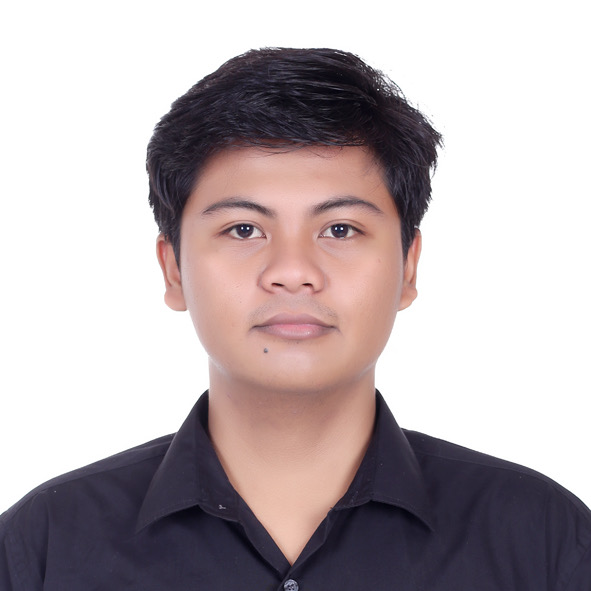
\includegraphics[width=\textwidth]{fix.jpg} % Mengatur lebar gambar agar sesuai
    \end{minipage}
    \hspace{5 mm} % Menambahkan spasi antara gambar dan konten di kanan
    & \begin{tabular}{@{}l@{}}
        \textbf{\Huge \scshape Jonathan Oktaviano Frizzy} \\[0.8em] % Jarak setelah nama
        \faMobile \hspace{.5pt} \href{wa.me/081357473781}{+62 813 5747 3781}
        $|$
        \faAt \hspace{.5pt} \href{mailto:jonathanoktavianofrizzy@gmail.com}{jonathanoktavianofrizzy@gmail.com} \\[0.1em] % Mengatur jarak antara baris
        \faLinkedinSquare \hspace{.5pt} \href{https://linkedin.com/in/jonathan-oktaviano/}{LinkedIn}
        $|$
        \faGithub \hspace{.5pt} \href{https://github.com/robotjaol}{GitHub}
        $|$
        \faGlobe \hspace{.5pt} \href{https://robotjaol.vercel.app/}{Portfolio}
        $|$
        \faMapMarker \hspace{.5pt} \href{https://maps.app.goo.gl/3KcJKWS8gMk1GiZMA}{Surabaya, Indonesia} \\
    \end{tabular}
\end{tabularx}
\vspace{1em}

%----------- EDUCATION -----------

% \section{Education}
%   \vspace{3pt}
%   \resumeSubHeadingListStart
    
%     \resumeEducationHeading
%       {Institut Teknologi Sepuluh Nopember}{Surabaya, Indonesia}
%       {1nd Year in Electrical Automation Engineering; \textbf{GPA: 3.49/4.00}}{Jul 2022 \textbf{--} Apr 2023}
      
    
  
%   \resumeSubHeadingListEnd

 \section{Education}
   \vspace{3pt} 
    \resumeSubHeadingListStart

       \resumeEducationHeading
         {Institut Teknologi Sepuluh Nopember}
         {Surabaya, Indonesia}
         {3nd Year in D4 Automation Electronic Engineering}
         {GPA: 3.55/4.00}
         {Jul 2022 -- Present}
  
    \resumeSubHeadingListEnd

%----------- EXPERIENCE -----------

\section{Experience}
  \vspace{3pt}
  \resumeSubHeadingListStart

    \resumeSubheading
      {PLC and Supervisory Control System Laboratory ITS}{Surabaya, Indonesia}
      {Member}{Dec 2022 \textbf{--} Present, Full-time}
        \resumeItemListStart
            \resumeItem{Studying programmable logic control, Control System Engineering, Industrial Robot and automation hierarchy, with a focus on industrial automation development.}
            \resumeItem{Focusing in Machine Vision, Monitoring, Automation Electricity, and Project Based Learning by Industry Factory or ITS}
        \resumeItemListEnd

    \resumeSubheading
      {Digital Talent Scholarship KOMINFO}{Surabaya, Indonesia}
      {Teaching Assistant}{Jan 2023 \textbf{--} Jun 2023, Part-time}
        \resumeItemListStart
            \resumeItem{Working on and evaluating the code submitted by participants Junior Website Developer.}
            \resumeItem{Compiling attendance data for each session.}
            \resumeItem{Conducting tests on each participant's Final Project, and then assigning assessment points to each feature of the projects submitted by the participants}
        \resumeItemListEnd


    \resumeSubheading
      {PT. Pertamina Trans Kontinental}{Cilacap, Indonesia}
      {Electrical Engineer}{Jun 2023 \textbf{--} Dec 2023, Full-time}
        \resumeItemListStart
            \resumeItem{Designed and developed electrical systems ensuring seamless integration with onboard communication tools.}
            \resumeItem{Spearheaded the design of power management solutions, including battery and energy storage systems.}
            \resumeItem{Provided expertise in communication systems and electrical architectures for oil navigation vessels.}
    \resumeItemListEnd

    \resumeSubheading
      {PT Innoveam}{Surabaya, Indonesia}
      {Electrical Engineer}{Jul 2024 \textbf{--} Aug 2024, Full-time}
        \resumeItemListStart
            \resumeItem{I work here as an electrical technician for target shooting robots at the Naval Military Academy shooting range. My responsibilities include creating electrical schematics, wiring, troubleshooting, and controlling each robot component using microcontrollers.}
    \resumeItemListEnd
    \vspace{2pt}
    \resumeSubheading
      {KKN Tematik Institut Teknologi Sepuluh Nopember}{Surabaya\textbf{--}Sidoarjo, Indonesia}
      {Leader}{Aug 2023 \textbf{--} Oct 2023, Part-time}
        \resumeItemListStart
            \resumeItem{Fully responsible as the project manager, overseeing the timeline, finances, and logistics in constructing the  \href{https://www.its.ac.id/news/2023/09/12/bantu-petambak-abmas-its-gagas-alat-pengontrol-kualitas-air/}{\color{blue}Smart Integrated Water Quality Monitoring System project}.}
            \resumeItem{Creating a monitoring device website using PHP to store data from all sensors of the device, accessible from anywhere.}
            \resumeItem{Designing the installation scheme of electronic hardware components for the project, comprising sensing components, actuators, and radio transmitters.}
        \resumeItemListEnd

      %    \resumeSubheading
      % {Wirausaha Merdeka ITS}{Surabaya, Indonesia}
      % {Electronics Engineer}{June 2023 \textbf{--} Oct 2023, Part-time}
      %   \resumeItemListStart
      %       \resumeItem{I designed and developed the electrical system for the "Beginner Kit Electronics" product using Autodesk Fusion 360 for the design and Proteus for circuit simulation. Additionally, I participated in business management training to meet specific business criteria and fulfill the requirements for the Free Entrepreneurship activity evaluation.  \href{https://www.youtube.com/watch?v=fzd8DhDGEHg}{\color{blue}Here is the documentation}.}
      %   \resumeItemListEnd

    \resumeSubheading
      {Barunastra ITS}{Surabaya, Indonesia}
      {Electrical Designer}{Dec 2022 \textbf{--} Present, Full-time}
        \resumeItemListStart
            \resumeItem{Developing an emergency control breaker system to enhance safety and reliability.}
            \resumeItem{Managing the placement and safety protocols of all electrical components within the robot to ensure optimal performance and compliance with safety standards.}
            \resumeItem{Designing the installation scheme of electronic hardware components for the project, comprising sensing components, actuators, and radio transmitters.}
        \resumeItemListEnd

        \resumeSubheading
      {Bioinformatics Study Club ITS}{Surabaya, Indonesia}
      {Vice Chairman}{June 2023 \textbf{--} Present, Part-time}
        \resumeItemListStart
            \resumeItem{As the Vice Chairman of the Bioinformatics Study Club, my responsibilities include Assisting the Chairman in overseeing club activities, ensuring smooth operation, and providing guidance to club members. Managing and coordinating research projects, workshops, and events to promote knowledge and skills in bioinformatics. \href{https://www.instagram.com/bsc.its/?hl=id}{\color{blue}Here is the instagram account}.}
        \resumeItemListEnd

    
  \resumeSubHeadingListEnd



%----------- AWARDS & ACHIEVEMENTS -----------

\section{Awards \& Achievements}
  \vspace{2pt}
  \resumeSubHeadingListStart
    \small{\item{
        \textbf{Autonomy Challenge at International Roboboat Competition:}{ Secured 3rd place by integrating and coordinating all electronic components in 'Nala Proteus V.2,' including PCB, sensors, and actuators. Developed electrical and communication architecture, implemented with a success rate of 90 percent {(Feb 2024)} \\ \vspace{3pt}
        
        \textbf{Autonomy Challenge at International Roboboat Competition:}{ 1st place, Working on and combining all electronic devices in "Nala Proteus" such as PCB and others.Designing electrical architecture and battery managament. {(Mar 2023)} \\ \vspace{3pt}
        
        \textbf{Autonomous Tourism Surface Vehicle Prototype Contest, (KKCTBN):}{ Secured the 1st place by Took part in helping on developing electrical systems for Barunastra ITS' "Nala Athena" Autonomous Tourism Surface Vehicle Prototype Ship. (Oct 2023)} \\ \vspace{3pt}
        
        \textbf{LKS Nasional Mobile Robotic:}{ Secured the 3rd place by creating a robot utilizing a National Instruments controller, MyRIO, integrated with actuators such as servos and PG motors, and featuring a camera for barcode, color, and obstacle detection, serving as a hospital service robot (Oct 2022)} \\ \vspace{3pt}
        
        % \textbf{SMK Sore Tulungagung Award:}{ Graduated as the highest ranked student.(Jun 2022)}
    }}}}
\resumeSubHeadingListEnd



%----------- PROJECTS -----------

\section{Projects}
    \vspace{3pt}
    \resumeSubHeadingListStart            
      \resumeProjectHeading
        {\textbf{Smart Integrated Water Quality Monitoring System} $|$ \emph{\href{https://www.its.ac.id/news/2023/09/12/bantu-petambak-abmas-its-gagas-alat-pengontrol-kualitas-air/}{\color{blue}Article}}}{}
          \resumeItemListStart
            \resumeItem{This project was part of my Community Empowerment Program (KKN), with a focus on thematic environmental issues. The primary goal was to monitor the water quality of ponds by measuring key parameters such as temperature, pH, and oxygen levels. To facilitate the analysis and sharing of this data, I also developed a website to store and display all the collected information. This project aimed to provide valuable insights into the environmental health of local water bodies and support efforts in maintaining and improving water quality.}
          \resumeItemListEnd

     \resumeProjectHeading
        {\textbf{PT. Pertamina Trans Kontinental "Oil Navigating Ship"} $|$ \emph{\href{https://www.linkedin.com/in/jonathan-oktaviano/details/projects/}{\color{blue}LinkedIn Experience}}}{}
          \resumeItemListStart
            \resumeItem{In this project, I assumed the dual role of an electrical and mechanical conceptor and consultant. My duties encompassed the design of electrical and communication diagrams for the ship, ensuring comprehensive and efficient systems integration. Additionally, I provided valuable recommendations for implementing ship maneuvers, contributing to the overall functionality and safety of the vessel. My multifaceted involvement underscores my expertise in both electrical and mechanical engineering disciplines, as well as my capacity to offer strategic insights across various aspects of maritime engineering projects.}
          \resumeItemListEnd
          
    \resumeSubHeadingListEnd

    
%----------- SKILLS -----------

\section{Skills}
  \vspace{2pt}
  \resumeSubHeadingListStart
    \small{\item{
        
        \textbf{Languages:}{ C/C++, C\#, Python, JavaScript, PHP, LabVIEW, MATLAB} \\ \vspace{3pt}
        
        \textbf{Technologies:}{ Flask, Streamlit, Node.js, React.js, Git, RabbitMQ, OpenCV, PyTorch, Mediapipe, TensorFlow, Arduino, ESP32, ESP8266, STM32, PLC Omron, PLC Mitsubishi, ROS2, KiCAD, Fusion360 CAD, Altium Designer} \\ \vspace{3pt}
        
        \textbf{Methodologies:} {OOP, Functional Programming, Kinematics, PID, Neural Network, CNN} \\ \vspace{3pt}
        
    }}
  \resumeSubHeadingListEnd


%----------- RELEVANT COURSEWORK -----------

% \section{Relevant Coursework}
%   \vspace{2pt}
%   \resumeSubHeadingListStart
%     \small{\item{
%         \textbf{Major coursework:}{ Materials Science, Electrical Circuits I-II, Digital System Design, Numerical Methods, Probability Theory, Electronics I-II, Signals and Systems, Electromagnetic Field Theory, Energy Conversion, System Dynamics and Control, Communication Engineering, Pattern Recognition, Introduction to Digital Signal Processing, Introduction to Digital Communications, Introduction to Database Systems, Introduction to Image Processing, Machine Vision} \\ \vspace{3pt}

%         \textbf{Minor coursework:}{ Discrete Computational Structures, Introduction to Object-Oriented Programming, Data Structures and Algorithms, Computer Organization, Fundamentals of Software Engineering}
%     }}
%   \resumeSubHeadingListEnd



%----------- CERTIFICATES -----------

\section{Certificates}
\resumeSubHeadingListStart
    \resumeOrganizationHeading
      {Project Manager by Google}{Mar 2024}{Foundation Project Management \href{https://www.coursera.org/account/accomplishments/verify/FUGNKUSUYHBA}{\color{blue}Certificate}.}

    \resumeOrganizationHeading
      {Artificial Intelligence for Business by NASBA}{Mar 2024}{Introduction to Artificial Intelligence \href{https://www.linkedin.com/in/jonathan-oktaviano/details/certifications/1710528282367/single-media-viewer/?profileId=ACoAAEB2k00Bw-v1yxcDJJYIGidC5SNJ_jZ5UHg}{\color{blue}Certificate}.}

    \resumeOrganizationHeading
      {CS50's Introduction to Artificial Intelligence with Python}{Aug 2024}{Artificial Intelligence (AI) and Python (Programming Language) by Harvard University. \href{https://www.linkedin.com/in/jonathan-oktaviano/details/certifications/}{\color{blue}Certificate}.}

  \resumeSubHeadingListEnd



%----------- ORGANIZATIONS -----------

\section{Organizations}
  \resumeSubHeadingListStart

    % \resumeOrganizationHeading
    %   {UKM Robotika ITS}{Oct 2022 -- Present}{Member}
      
    \resumeOrganizationHeading
      {Barunastra ITS}{Dec 2022 -- Present}{Expert Staff Electrical Division}

    \resumeOrganizationHeading
      {Bioinformatics Study Club ITS}{May 2024 -- Present}{Vice Chairman}

  \resumeSubHeadingListEnd



%----------- HOBBIES -----------

% \section{Hobbies}
  % \resumeSubHeadingListStart
    % \small{\item{Basketball, Swimming, Fitness, Eight-ball, Horology}}
  % \resumeSubHeadingListEnd



%----------- REFERENCES -----------

% \section{References}
  % \vspace{2pt}
  % \resumeSubHeadingListStart
    % \item{References available upon request.}
  % \resumeSubHeadingListEnd



%-------------------------------------------
\end{document}